\documentclass[aspectratio=169,11pt]{beamer}
\usepackage{assets/agrawal-beamer}

\title[Agrawal et al. (2025)]{The Economics of Bicycles for the Mind}
\subtitle{Herramientas cognitivas, esfuerzo y desigualdad}
\author{Belén Vásquez}
\institute{Universidad del Pacífico}
\date{Agosto de 2026}

\begin{document}

\begin{frame}[plain]
  \titlepage
  \vspace{-0.8em}
  \begin{center}
    \small \paperref\\[0.45em]
    \href{\RepoURL}{\texttt{github.com/sbvasquezg-ux/ai-02-agrawal}}
  \end{center}
\end{frame}

\begin{frame}{1 \textperiodcentered{} Una cadena de mejoras con tres capacidades}
  \textbf{Pregunta.} ¿Cómo cambian las herramientas cognitivas el esfuerzo,
  la productividad y la desigualdad cuando sustituyen implementación pero
  complementan juicio?

  \medskip
  \textbf{Mecanismo único.} Encontrar una oportunidad $\to$ intentar
  implementarla $\to$ continuar si aparece otra.

  \medskip
  \begin{columns}[T,onlytextwidth]
    \column{0.62\textwidth}
    \textbf{Problema condicional en una oportunidad}
    \[
      e_t^*(\theta)\in\arg\max_{e_t\ge0}
      \{\alpha\Delta p(se_t;\theta)-c(e_t;\theta)\}.
    \]
    \textbf{FOC interior}
    \[
      \alpha\Delta s\,p'(se_t^*;\theta)=c'(e_t^*;\theta).
    \]
    \column{0.35\textwidth}
    \keybox{\small
      $s$: implementación\\[0.35em]
      $\alpha$: juicio de resultado\\[0.35em]
      $\gamma(t)$: juicio de oportunidad
    }
  \end{columns}

  \smallskip
  \footnotesize Elección: $e_t$. Restricción: $e_t\ge0$. Tecnología:
  $p\in[0,1]$ creciente y cóncava; $c$ creciente y convexa.
  \sourcefoot{\paperref, secciones 3.1--3.3.}
\end{frame}

\begin{frame}{2 \textperiodcentered{} Las tres proposiciones: resultados}
  \footnotesize
  \begin{block}{Proposición 1 \textperiodcentered{} Esfuerzo y productividad}
    Al adoptar la herramienta, el esfuerzo óptimo cae en cada ronda,
    $e_t^*(1)<e_t^*(0)$; es igual entre rondas tecnológicamente idénticas; y el
    valor esperado total aumenta, $V_0(1)>V_0(0)$.
  \end{block}

  \begin{block}{Proposición 2 \textperiodcentered{} Quién gana más con la adopción}
    La ganancia aumenta con el juicio de oportunidad; aumenta con $\alpha$ si la
    adopción eleva la probabilidad de éxito realizada; disminuye con $s$ bajo
    sustitución suficientemente fuerte; y pesa más cuando la oportunidad llega
    temprano. Las dos últimas comparativas requieren las cautelas de la auditoría.
  \end{block}

  \begin{block}{Proposición 3 corregida \textperiodcentered{} Media y desigualdad}
    Bajo la tecnología especializada, independencia, $\delta\gamma<1$, momentos
    finitos y un rango interior común, $\mathbb E[V(\theta)]$ aumenta. Si además
    $\operatorname{Var}(\Gamma/s)>0$ y
    $\mathbb E[\Gamma^2]/\mathbb E[\Gamma]^2<\mu_s\mathbb E[1/s]$, la varianza
    transversal $\operatorname{Var}[V(\theta)]$ es convexa: cae hasta $\theta^*$
    y sube después; que ya suba en $\theta=1$ exige $\alert{\theta^*<1}$.
  \end{block}
  \sourcefoot{\paperref, Proposiciones 1--3 y apéndices; correcciones propias.}
\end{frame}

\begin{frame}{3 \textperiodcentered{} Qué verifiqué a mano y por qué}
  \begin{columns}[T,onlytextwidth]
    \column{0.57\textwidth}
    \small
    \begin{block}{De la suma general a la ecuación (23)}
      Partí de la ecuación (21). Por la Proposición 1,
      $e_t^*(\theta)=e^*(\theta)$; además,
      $\gamma(0)=\gamma_0$ y $\gamma(t)=\gamma$ para $t\ge1$. Entonces
      \[
        \begin{aligned}
        V_0(\theta)
          &=\gamma_0M(e^*(\theta);\theta)
            \sum_{t=0}^{\infty}(\delta\gamma)^t\\
          &=\frac{\gamma_0M(e^*(\theta);\theta)}{1-\delta\gamma},
            \qquad \delta\gamma<1.
        \end{aligned}
      \]
    \end{block}
    \keybox{\small Elegí esta parte porque sostiene la Proposición 1, reaparece
    en la 2 y ofrece una prueba autocontenida, sin imponer formas específicas
    para $p(\cdot)$ o $c(\cdot)$.}

    \column{0.39\textwidth}
    \begin{center}
      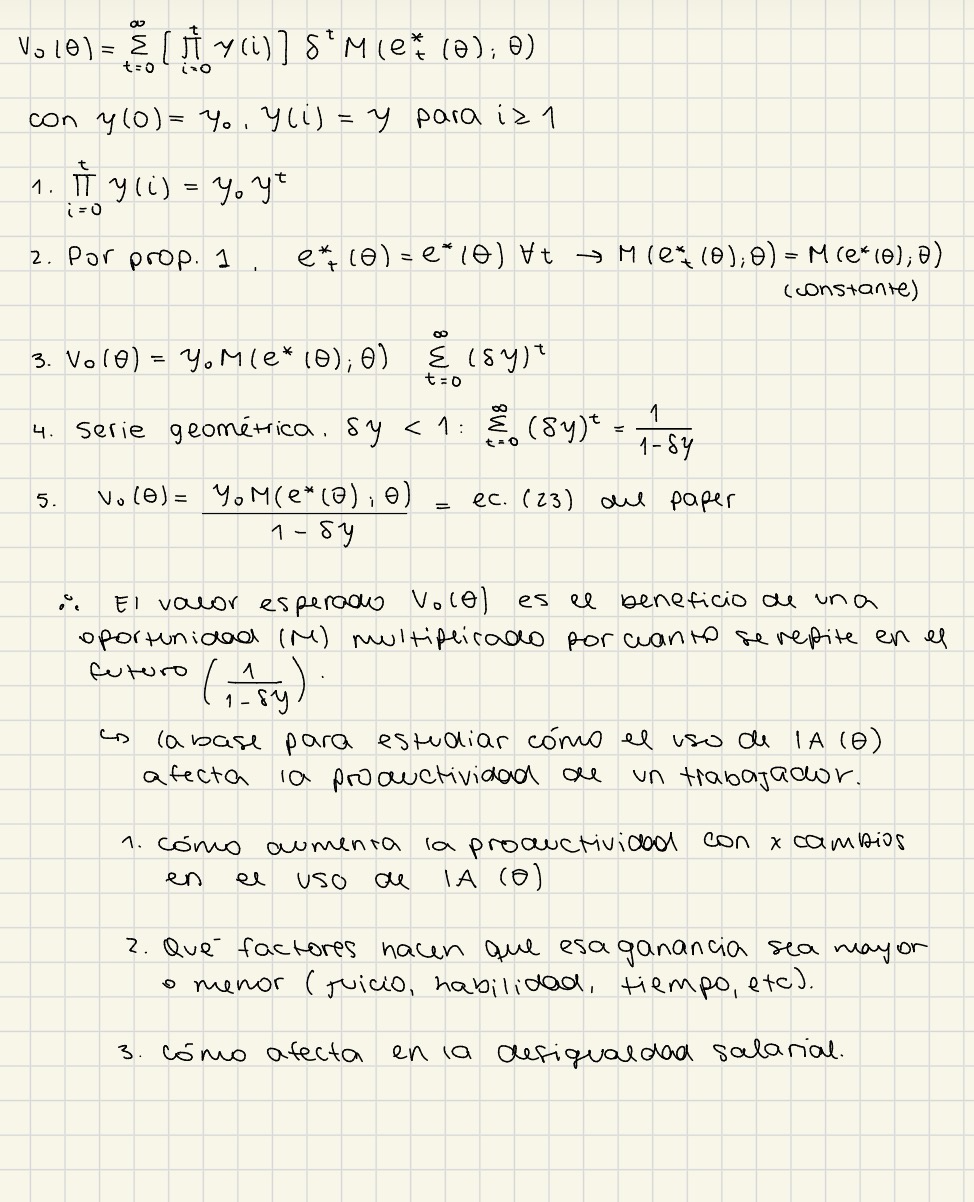
\includegraphics[width=\linewidth,height=0.68\textheight,keepaspectratio]{hand/manual-verification.png}
      \par\scriptsize Verificación manual de la ecuación (23).
    \end{center}
  \end{columns}
  \sourcefoot{Elaboración propia a partir de \paperref, ecuaciones (21) y (23).}
\end{frame}

\begin{frame}{4 \textperiodcentered{} Qué nos dice esta derivación}
  \begin{block}{Interpretación económica}
    \[
      V_0(\theta)
      =\underbrace{\gamma_0M(e^*(\theta);\theta)}_{\text{beneficio de la oportunidad inicial}}
      \times
      \underbrace{\frac{1}{1-\delta\gamma}}_{\text{repetición futura}}.
    \]
  \end{block}

  \begin{block}{Su rol en el paper}
    Es el bloque base para estudiar cómo la adopción de la herramienta afecta
    la productividad: la Proposición 1 pregunta si sube el valor esperado; la 2,
    qué factores amplifican la ganancia; y la 3, cómo cambia la varianza entre
    trabajadores.
  \end{block}

  \keybox{\textbf{Veredicto.} La forma cerrada queda confirmada por la serie
  geométrica: no es un resultado inventado por la IA.}
  \sourcefoot{Verificación manual propia; \paperref, ecuaciones (21) y (23).}
\end{frame}

\end{document}
